\chapter{Sistema mínimo}
\label{C:SistemaMinimo}
El primer circuito diseñado para el desarrollo del trabajo fue el \textbf{Sistema Mínimo}, un sistema simplificado que consta de una arquitectura simple, con el objetivo de analizar el funcionamiento del microprocesador y el uso del mapa de memoria. Este sistema consta de dos grandes bloques como se observa en la figura~\ref{F:diag_bloq_sistema_minimo}: el microprocesador y la memoria. 

\begin{figure}[ht]
  \centering
  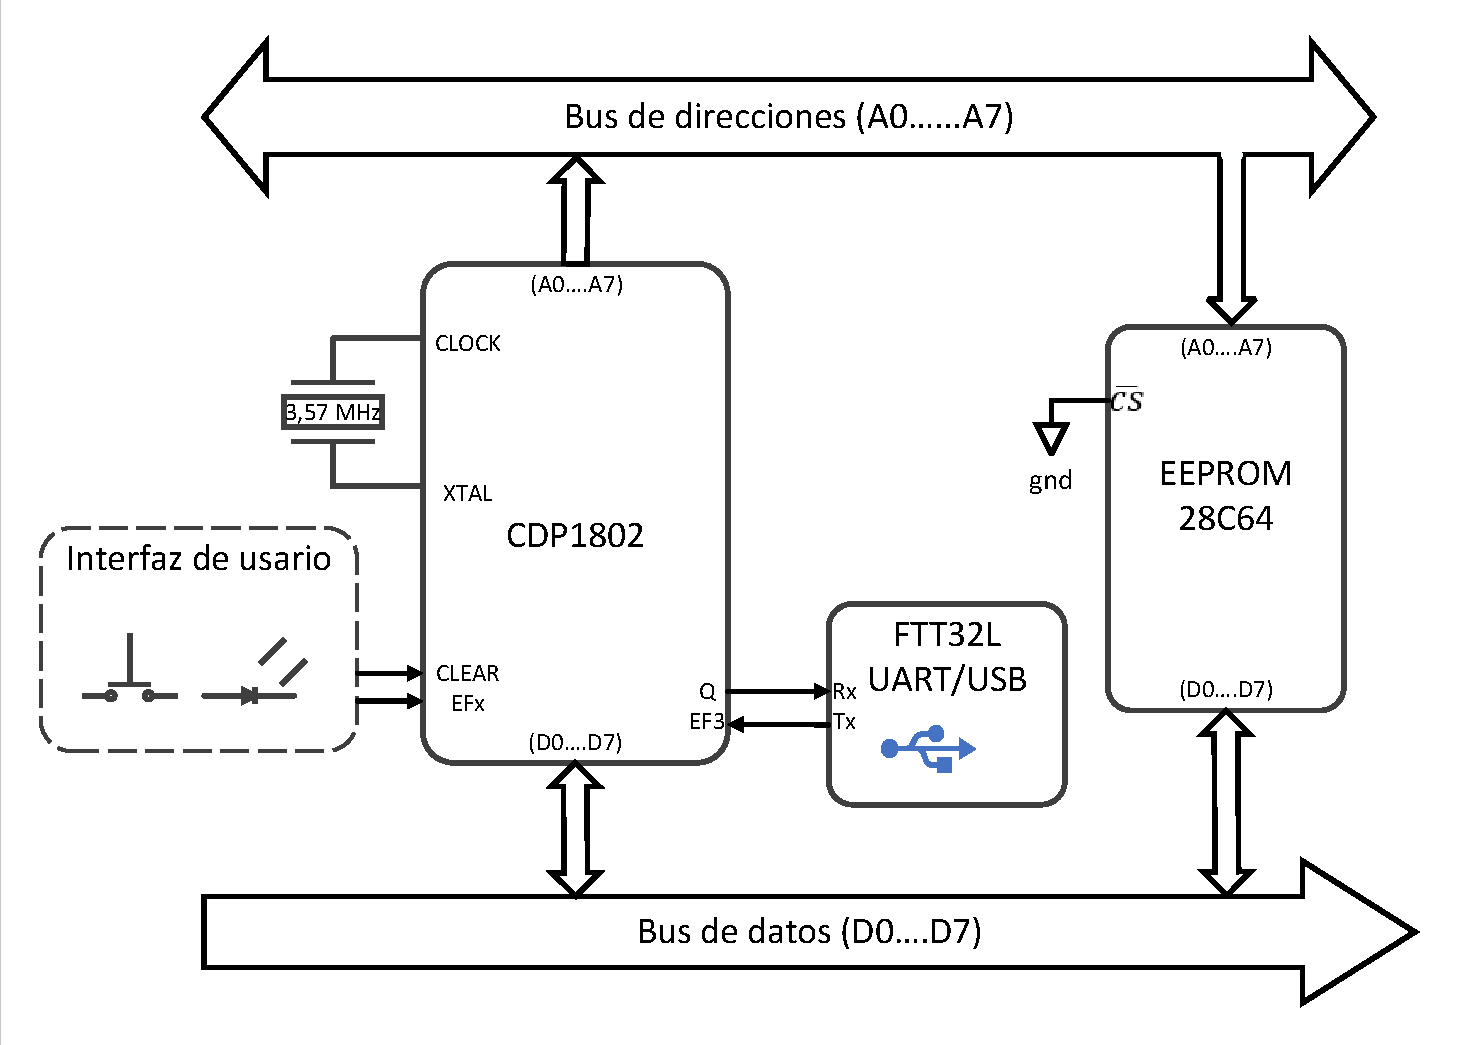
\includegraphics[width=0.9\textwidth]{./imagenes/diag_bloq_sistema_minimo.pdf}
  \caption{Diagrama de bloques del sistema mínimo}
  \label{F:diag_bloq_sistema_minimo}
\end{figure}

El microprocesador es el elemento central del circuito diseñado, que es donde se realiza todo el procesamiento de datos. La incorporación del mismo permite realizar pruebas de funcionamiento, facilitando el entendimiento del lenguaje de programación y la secuencia de las instrucciones y ejecución dentro del microprocesador. Por otro lado, la memoria dentro de este sistema cumple la función de almacenar las instrucciones del programa a ejecutar y no se utiliza la misma para guardar datos generados en ejecución. Debido a la simplicidad del sistema presentado y la arquitectura del microprocesador, solo se utilizó un direccionamiento de 8 bits, lo que limita el tamaño del programa principal a un máximo de 256 bytes. Esto se debe a que el direccionamiento de 16 bits requiere el agregado de más elementos al circuito lo cual se explica en el desarrollo del sistema medio en la sección~\ref{C:SistemaMedio}. Con esta arquitectura los programas desarrollados debían ser simples con el único objetivo de determinar y comprobar el correcto funcionamiento de las conexiones y lograr un entendimiento básico del lenguaje de programación y del microprocesador. Para este fin se utilizan los programas desarrollados y presentados en la sección~\ref{C:ProgramasSMin}.

Debido a las limitaciones en el direccionamiento, se dispuso un diseño que permite establecer el estado de los pines de dirección A8 y A9 de la memoria de programa (28C64), directamente sobre el chip. Esto permite utilizar cuatro sectores de la memoria, aunque no simultáneamente. El microprocesador sigue utilizando únicamente 8 bits para el direccionamiento de memoria. Para la modificación se utilizan puentes tipo jumper que permiten conectar a masa o a VCC tanto A8 como A9 individualmente. De esta forma se establece un mapa de memoria como el presentado en la figura~\ref{F:Mapa_SMin}. De esta manera al realizar el grabado de la memoria EEPROM se pueden incluir los cuatro programas presentados en la sección \ref{C:ProgramasSMin} y pueden ser probados sin necesidad de regrabar la memoria.

\begin{figure}[ht!]
\centering
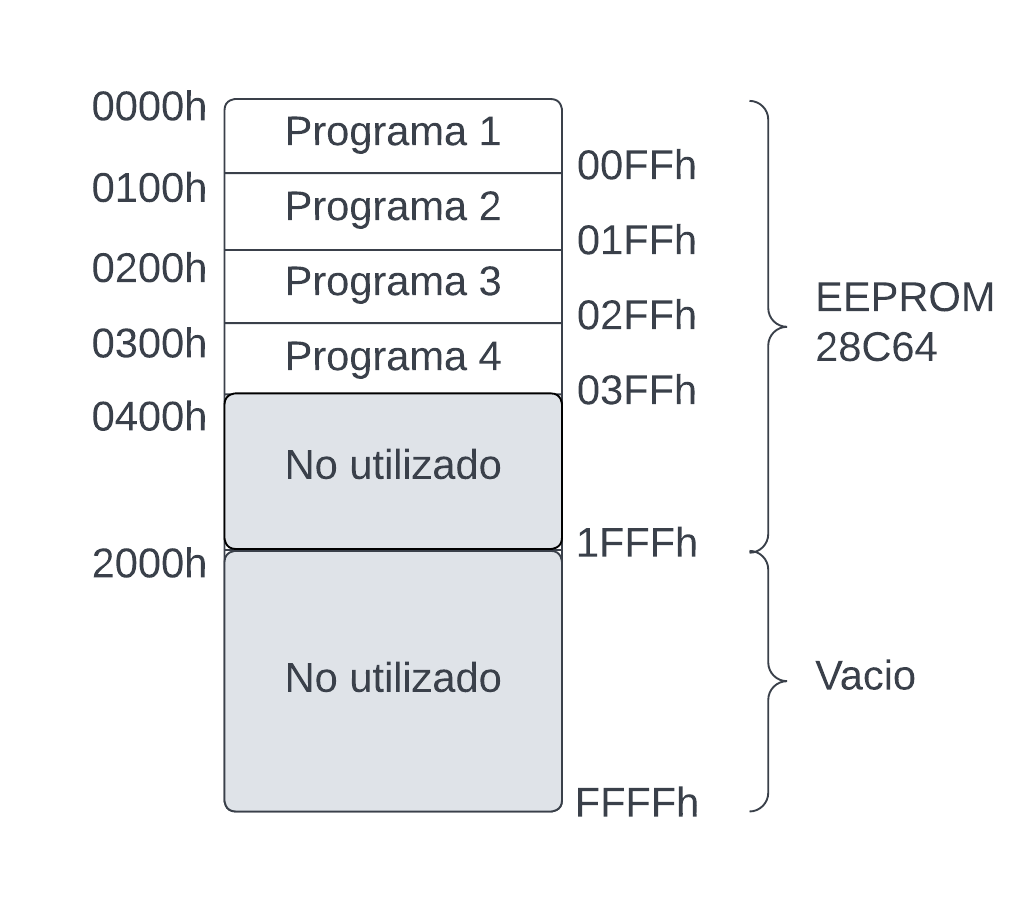
\includegraphics[width=0.57\textwidth]{./imagenes/Mapa_SMin.png}
\caption{\centering Mapa de memoria Sistema Mínimo}
\label{F:Mapa_SMin}
\end{figure}

\clearpage
Para elegir cada uno de los programas debe conectarse adecuadamente un jumper en los conectores de J10 y otro jumper en los conectores de J11, como se describe a continuación.

\begin{description}
    \item[Programa 1:] Conectar un jumper en los pines 2 y 3 de J10, y otro jumper en los pines 2 y 3 de J11.
    \item[Programa 2:] Conectar un jumper en los pines 1 y 2 de J10, y otro jumper en los pines 2 y 3 de J11. 
    \item[Programa 3:] Conectar un jumper en los pines 2 y 3 de J10, y otro jumper en los pines 1 y 2 de J11. 
    \item[Programa 4:] Conectar un jumper en los pines 1 y 2 de J10, y otro jumper en los pines 1 y 2 de J11. 
\end{description}

Para que el circuito funcione correctamente se implementó un sistema de alimentación basado en un regulador de tensión de 5~V, específicamente el UTC7805. La incorporación del mismo proporciona mayor estabilidad en la alimentación protegiendo a los circuitos integrados del sistema. También se incorporó una interfaz de usuario simple que consta de pulsadores como sistema de entrada y LED indicadores de funcionamiento. 

Para la realización del esquemático y el diseño de la placa PCB se utilizó el programa KiCad. El esquema obtenido se presenta en la figura~\ref{F:EsquemaSMin}, además se lo presenta en el apéndice donde se encuentra en tamaño original. La placa PCB diseñada es una simple faz, la pista generada se presenta en la figura~\ref{F:PistaSMin}, mientras que la máscara de componentes de la misma se presenta en la figura~\ref{F:MascaraSMin}.

\begin{figure}[ht]
  \centering
  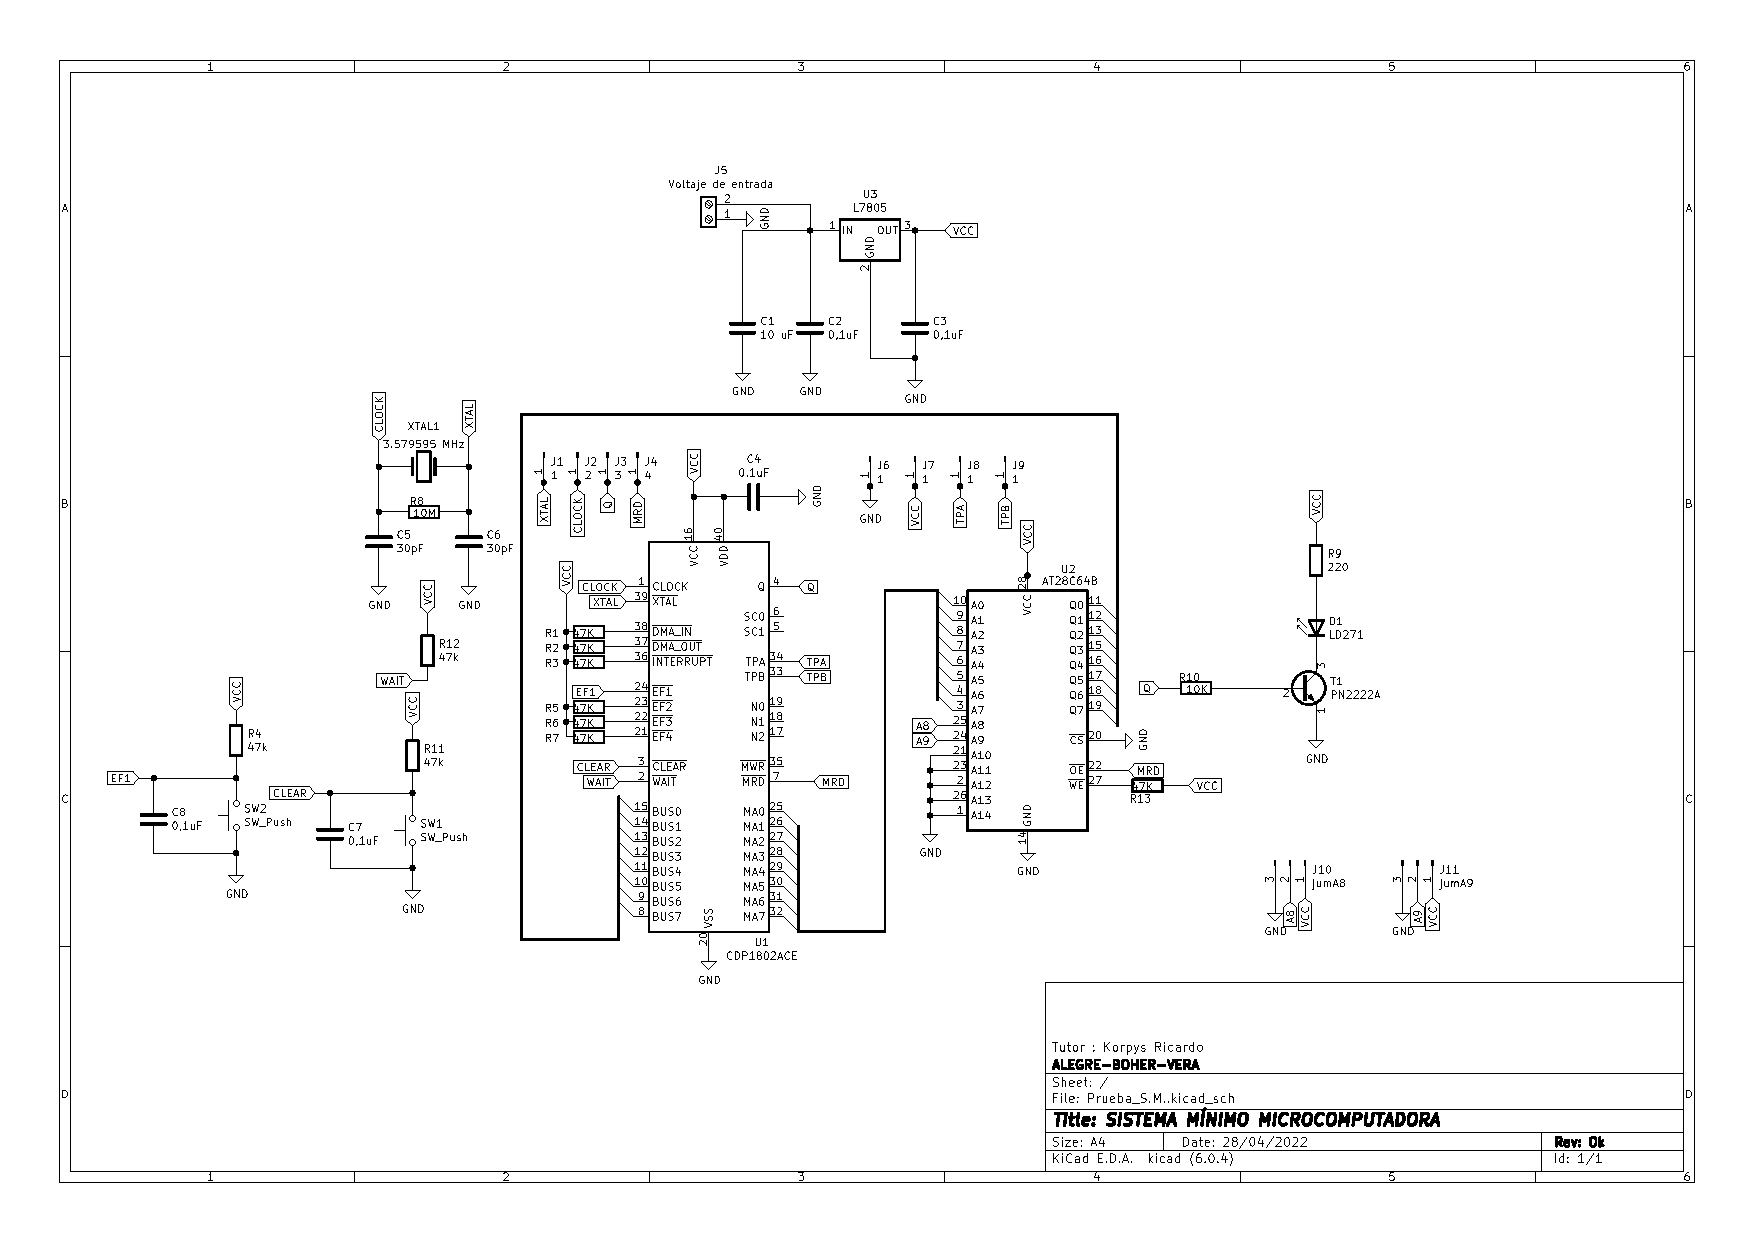
\includegraphics[width=1.2\textwidth, angle=90]{./imagenes/Esq_S.Min..pdf}
  \caption{Esquema de sistema mínimo}
  \label{F:EsquemaSMin}
\end{figure}




\begin{figure}[ht]
\centering
\subfloat[Pista diseñada para sistema mínimo]{
	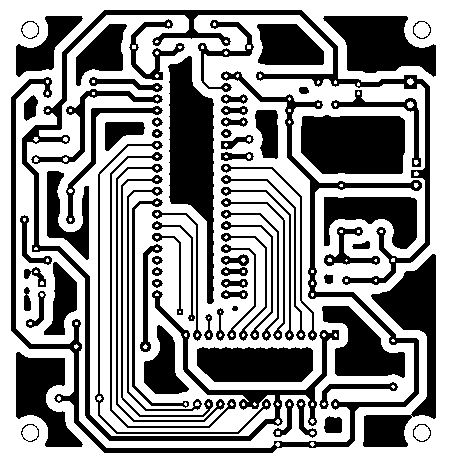
\includegraphics[width=0.52\textwidth]{./imagenes/PistaSMin.png}
	\label{F:PistaSMin}}

\subfloat[Máscara de componentes sistema mínimo]{
	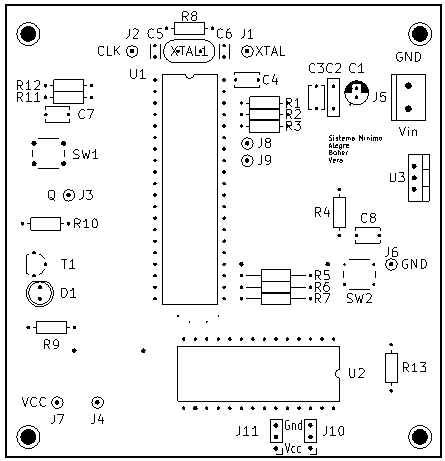
\includegraphics[width=0.51\textwidth]{./imagenes/MascaraSMin.png}
	\label{F:MascaraSMin}}
\caption{Placa PCB diseñada para sistema mínimo}
\label{F:PlacaPCB}
\end{figure}

\clearpage

A partir de los diagramas presentados se procedió a la construcción del circuito. El resultado obtenido se presenta en la fotografía~\ref{F:SMin}. El mismo funcionó correctamente sin necesidad de realizar modificaciones a la arquitectura propuesta. Sin embargo, para la prueba de transmisión de datos mediante UART, con el programa que se presentará en la sección~\ref{C:ComunicacionSerial}, se utilizó una interfaz externa para la conversión del sistema UART a USB, esto permite la recepción de la información en una terminal. La interfaz utilizada es el circuito FT232RL\cite{datasheet_FT232RL}, la cual fue contemplada para los diseños posteriores al sistema mínimo. 

\begin{foto}[ht]
  \centering
  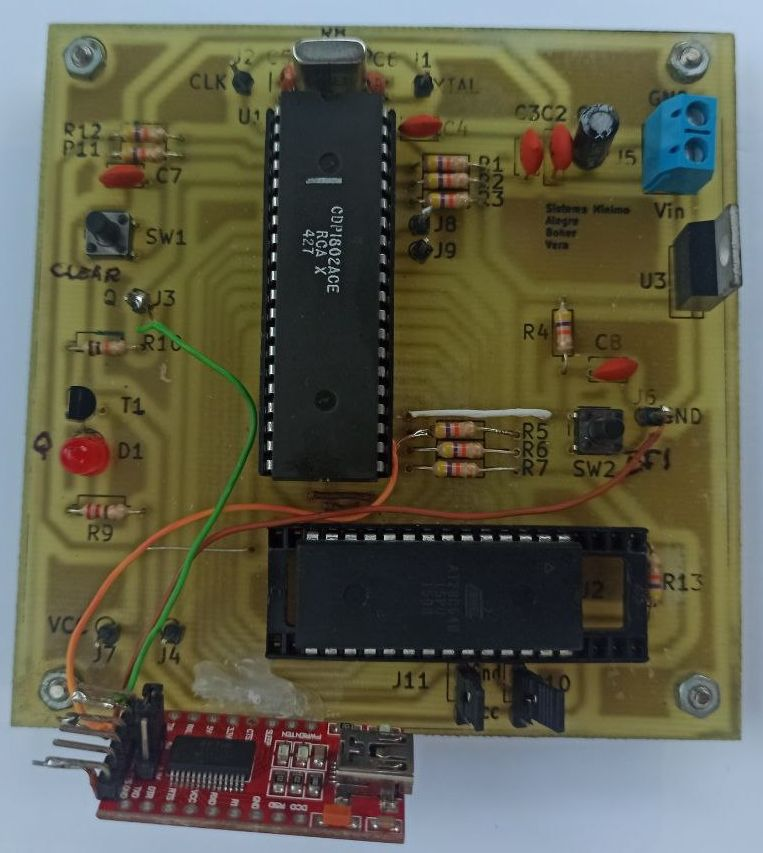
\includegraphics[width=0.5\textwidth]{./imagenes/foto_sistema_min.jpg}
  \caption{Sistema mínimo construido}
  \label{F:SMin}
\end{foto}

\clearpage
\section{Lista de componentes}

En la tabla~\ref{T:bom_sis_min} se encuentra la lista de materiales para la construcción del sistema mínimo.

\begin{table}[ht!]
\caption{Lista de componentes del sistema mínimo}
\label{T:bom_sis_min}
\footnotesize
\begin{tabular}{|p{0.08\textwidth}|p{0.11\textwidth}|p{0.30\textwidth}|p{0.14\textwidth}|p{0.15\textwidth}|}
\hline
Cantidad & Etiqueta \newline
           Identificador            & Descripción                               & Fabricante            & Número de parte \\ \hline \hline
1       & U1                        & Microprocesador                           & RCA                   & CDP1802ACE      \\ \hline
1       & U2                        & Memoria EEPROM 8k x 8                     & ATMEL                 & AT28C64B          \\ \hline
1       & U3                        & Regulador de tensión                      & YOUW ANG              & UTC7805          \\ \hline
1       & T1                        & Transistor BJT NPN                        & ST Microelectronics   & PN2222A           \\ \hline
1       & XTAL1                     & Cristal \num{3.579545}~\si{\mega\hertz}   & CQ Electronics        & \listaVacio                \\ \hline
2       & SW1, SW2                  & Pulsador 6mm~x~4,3mm                      & \listaVacio           & \listaVacio       \\ \hline
10      & R1, R2, R3, R4, R5, R6, R7, R11, R12, R13
                                    & Resistor 47~\si{\kilo\ohm} 1/8~\si{\watt} & \listaVacio                      & \listaVacio                \\ \hline
1       & R8                        & Resistor 10~\si{\mega\ohm} 1/8~\si{\watt} & \listaVacio                      &    \listaVacio             \\ \hline
1       & R9                        & Resistor 220~\si{\ohm} 1/4~\si{\watt}     & \listaVacio                      &    \listaVacio             \\ \hline
1       & R10                       & Resistor 10~\si{\kilo\ohm} 1/8~\si{\watt} &  \listaVacio                     &  \listaVacio               \\ \hline
1       & D1                        & LED Rojo 5mm                              & \listaVacio                      &  \listaVacio               \\ \hline
1       & C1                        & Capacitor electrolítico 10~\si{\micro\farad} 25~\si{\volt}
                                                                                &  \listaVacio                     &   \listaVacio              \\ \hline
5       & C2, C3, C4, C7, C8        & Capacitor cerámico \num{0.10}~\si{\micro\farad} 50~\si{\volt}
                                                                                &  \listaVacio                     & \listaVacio                \\ \hline
2       & C5, C6                    & Capacitor cerámico \num{30}~\si{\pico\farad} 50~\si{\volt}
                                                                                & \listaVacio                      & \listaVacio                \\ \hline
8       & J1, J2, J3, J4, J6, J7, J8, J9
                                    & Pin conector macho (1 \textit{Male Header Pin})
                                                                                & \listaVacio                      &  \listaVacio               \\ \hline
1       & J5                        & Bornera 2 pines \num{5.08}~mm             & \listaVacio                      &  \listaVacio               \\ \hline
2       & J10, J11                  & 1x3 Pines Conectores Macho \num{2.54}~mm        & \listaVacio                      & \listaVacio                \\ \hline
\end{tabular}
\normalsize
\end{table}

Algo no contemplado en esta lista de componentes es el módulo FT232RL~\cite{datasheet_FT232RL}, dado que fue soldado luego de armado el circuito, como puede apreciarse en la figura~\ref{F:SMin}. El módulo FT232RL tiene soldado con cables sus pines Rx, Tx, Vcc y GND, a los pines Q, EF2, Vcc y GND del microprocesador, respectivamente.

%%-------------------------------------------------------------------------------------------

\clearpage
\section{Programas del sistema mínimo}
\label{C:ProgramasSMin}
Para probar el sistema mínimo, se confeccionaron cuatro programas sencillos de no más de 256 bytes, debido a que el sistema mínimo no puede direccionar más que esta cantidad de direcciones de memoria. Los programas se presentan a continuación, haciendo uso de diagramas de flujo. Sin embargo, en el apéndice~\ref{C:anexo-programas-sistema-mínimo} se encuentra el código fuente de los cuatro programas.

\subsection{Programa 1: Parpadeo LED Q}

El primer programa hace parpadear el LED conectado a la salida Q del microprocesador. Para ello, como puede apreciarse en el diagrama de flujo de la figura~\ref{F:prog_1}, el programa comienza apagando el LED (Q~=~0), luego realiza un retardo por software, que consiste en la asignación de un valor específico a un registro, para luego decrementarlo hasta que llegue a cero. Una vez finalizado el retardo, el LED togglea; si está encendido, se apaga, y si está apagado, se enciende. Esta secuencia se repite constantemente, haciendo parpadear el LED conectado a la salida Q. En el apéndice~\ref{C:anexo-prog-1}, se encuentra el código fuente del programa~1.

\begin{figure}[ht]
  \centering
  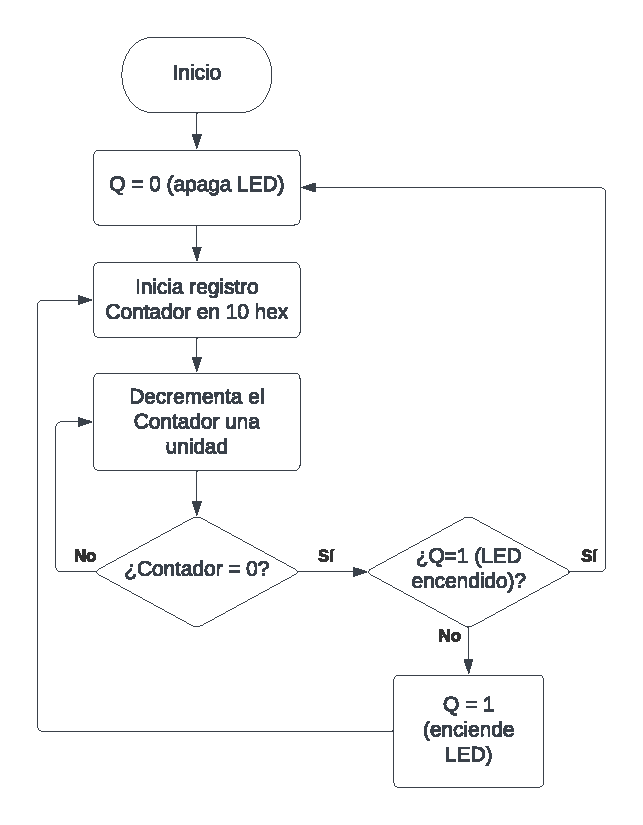
\includegraphics[width=0.5\textwidth]{./imagenes/programa_1.pdf}
  \caption{Programa 1}
  \label{F:prog_1}
\end{figure}

\clearpage
\subsection{Programa 2: LED Q se enciende al presionar pulsador}

El programa dos permite al usuario interactuar con el sistema, de manera que se prueba el funcionamiento de las entradas EFx (en el caso del sistema mínimo, EF1, dado que allí se encuentra conectado el pulsador). En el diagrama de flujo de la figura~\ref{F:prog_2} se puede observar cómo opera el programa. Cuando el botón se encuentra presionado, el programa entra a un bucle infinito que ejecuta el comando para encender el LED, en caso contrario, el programa entra a un bucle similar, pero donde la instrucción que se ejecuta continuamente es la de apagado del LED. En el apéndice~\ref{C:anexo-prog-2}, se encuentra el código fuente del programa~2.

\begin{figure}[H]
  \centering
  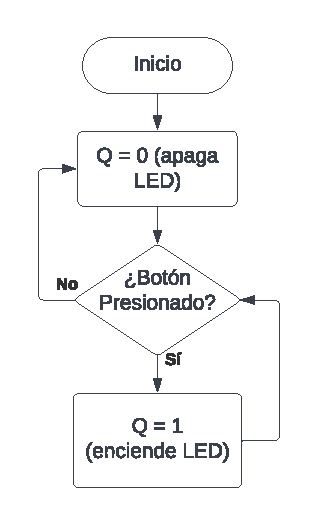
\includegraphics[width=0.3\textwidth]{./imagenes/programa_2.pdf}
  \caption{Programa 2}
  \label{F:prog_2}
\end{figure}

\clearpage
\subsection{Programa 3: LED Q parpadea al presionar pulsador}

El programa 3 es una combinación de los dos programas previos, el mismo hace parpadear el LED conectado a la salida Q del microprocesador, pero lo hace solo si el usuario presiona el pulsador.

En la figura~\ref{F:prog_3} se encuentra el diagrama de flujo del programa, el mismo consiste de una rutina de retardo con un contador que disminuye hasta cero (como en el programa 1), y luego, si el pulsador se encuentra presionado, el LED comienza a parpadear, pero si el pulsador no se encuentra presionado, el LED permanece apagado. En el apéndice~\ref{C:anexo-prog-3}, se encuentra el código fuente del programa 3.

\begin{figure}[H]
  \centering
  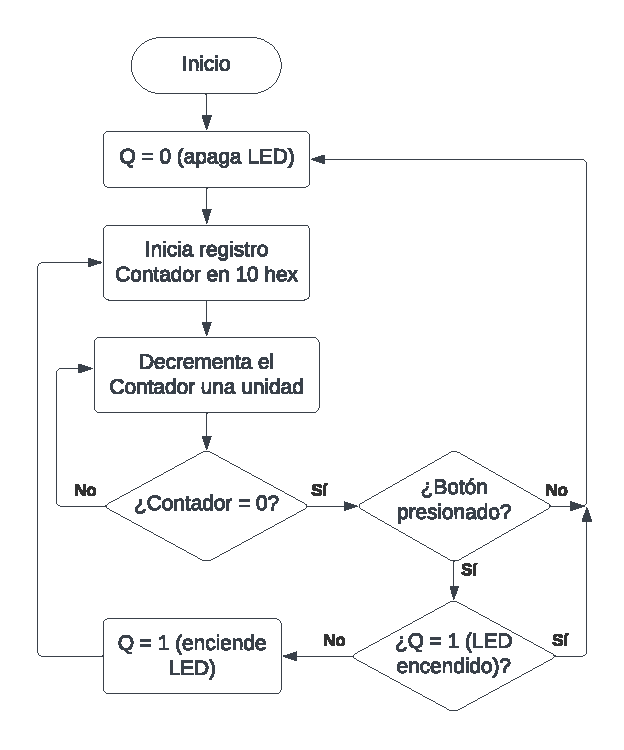
\includegraphics[width=0.6\textwidth]{./imagenes/programa_3.pdf}
  \caption{Programa 3}
  \label{F:prog_3}
\end{figure}

\clearpage
\subsection{Programa 4: Transmisión serial de caracteres}
\label{C:ComunicacionSerial}

El programa 4 realiza la transmisión serial por protocolo UART a través del pin Q de los caracteres “ABCDEFG”, seguido de un retorno de carro y un salto de línea. Este es el más complejo de los programas confeccionados para el sistema mínimo, por lo tanto, se encuentra descripto en dos diagramas de flujo separados, uno para la rutina principal, figura~\ref{F:prog_4_main} y otro para la rutina de transmisión de datos, figura~\ref{F:prog_4_rut_trans}. Si es de interés para el lector, en el apéndice~\ref{C:anexo-prog-4} se encuentra el código fuente.

 En la rutina principal, figura~\ref{F:prog_4_main}, inicialmente se inicializa el registro Contador  (en 7 decimal), que se utiliza para realizar la misma rutina 7 veces, y el registro Carácter (en 65 decimal), el cual representa el carácter A del código ASCII. Luego se ejecuta un bucle 7 veces seguidas, utilizando para ello el registro Contador. El mismo se decrementa una unidad en cada repetición del bucle y al llegar a cero en la última repetición, el programa sigue con su rutina. Dentro del bucle, Carácter es asignado a otro registro denominado Dato\footnote{Esta asignación parece a primera vista redundante, pero la razón de ello es que la rutina de trasmisión modifica el registro Dato, por lo tanto, se requiere que el dato a trasmitir permanezca guardado en otro lado, en este caso en el registro Carácter.}, en este registro debe encontrarse el dato a ser transmitido por la rutina de transmisión, seguidamente se llama a esa rutina, enviando el primer carácter (letra A). Seguidamente se llama a una rutina de retardo, se incrementa Carácter (pasando al siguiente carácter ASCII) y se vuelve a transmitir. Luego de ejecutarse 7 veces este bucle, se han transmitido los caracteres “ABCDEFG”.

A continuación, se sale del bucle y se envían los caracteres retorno de carro (D hexadecimal en codificación ASCII) y salto de línea (A hexadecimal en codificación ASCII). Esto concluye la rutina principal, la cual, al finalizar, vuelve a ejecutarse desde el comienzo.

En cuanto a la rutina de transmisión, figura~\ref{F:prog_4_rut_trans}, la misma envía los datos de forma serial por protocolo UART utilizando para ello el pin Q del microprocesador como salida de transmisión. En el apéndice~\ref{C:anexo-comunicación-serial} (\nameref{C:anexo-comunicación-serial}) se encuentran explicados los detalles relacionados con este protocolo.

La rutina de transmisión comienza pasando el pin Q de su estado de reposo (Q~=~1) a estado bajo (Q~=~0) por un periodo de 1~bit-time, este es el bit de inicio de la trama UART. Luego se inicializa un contador en 8 decimal, para realizar un bucle que se repite 8 veces, una por cada bit del dato de 8 bits. En este bucle el dato a enviar se corre a la derecha, cargando el LSB en el bit DF interno del microprocesador, en base al valor de este bit, se decide si poner la línea en estado alto (Q~=~1) o bajo (Q~=~0). Esto se repite 8 veces, de manera tal que se envían todos los bits del dato, del LSB al MSB. Finalmente se envían dos bits de parada (Q~=~1) para terminar la transmisión del dato.

\begin{figure}[H]
\centering
\subfloat[Rutina principal]{
	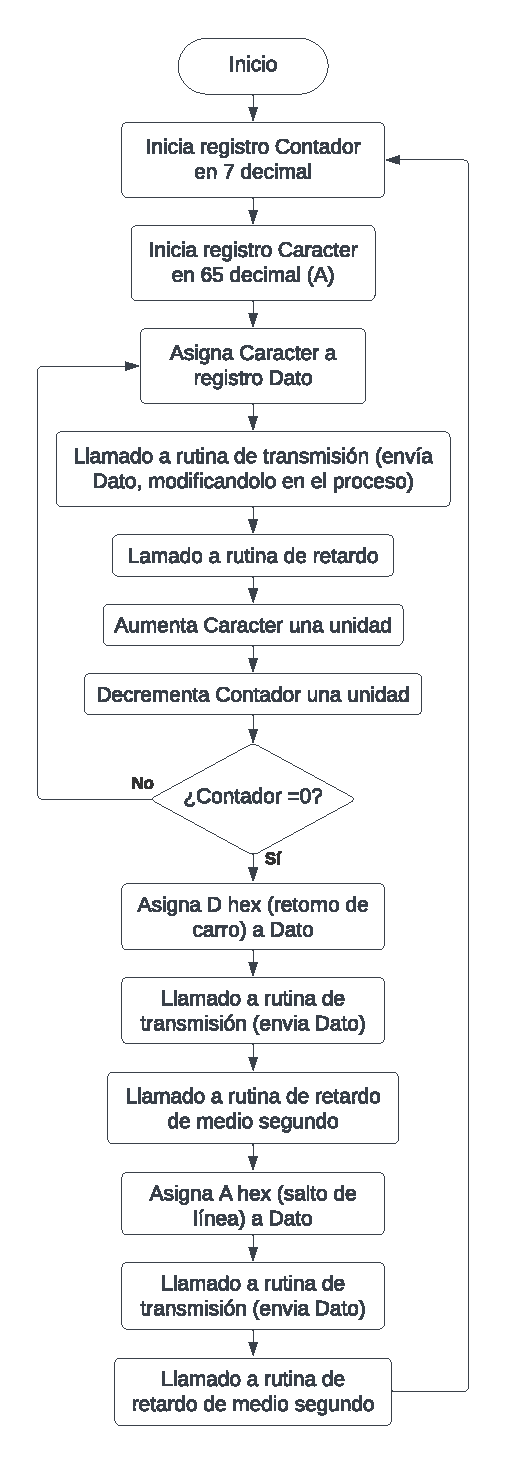
\includegraphics[width=0.45\textwidth]{./imagenes/programa_4_main.pdf}
	\label{F:prog_4_main}}
\quad
\subfloat[Rutina de transmisión]{
	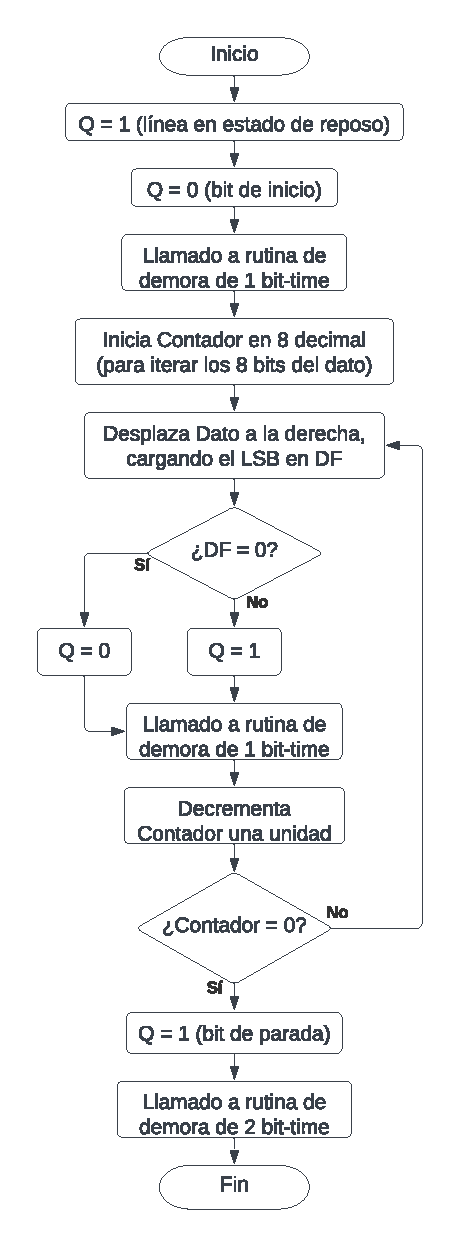
\includegraphics[width=0.45\textwidth]{./imagenes/program_4_rut_de_trans.pdf}
	\label{F:prog_4_rut_trans}}
\caption{Programa 4}
\label{F:prog_4}
\end{figure}

El programa 4 cuenta con muchas subrutinas, todas ellas fueron escritas con el método denominado \entreComillas{SEP technique}, el cual se encuentra descrito, junto a otros métodos, en la página 130 del libro Design Ideas Book for the CDP1802 COSMAC Microprocessor\cite{cdp1802_design_ideas}. El método SEP para las subrutinas fue utilizado por no requerir RAM para su operación, algo necesario, dado que el sistema mínimo no posee RAM.

En el listado~\ref{L:retardo}, se encuentra la rutina de retardo de un bit-time. En cada línea, como comentario, está indicado, para cada instrucción, el número de bytes, el número de ciclos máquina y la cantidad de veces que se ejecuta cada instrucción al llamarse la rutina. Esta información nos permite determinar el retardo ocasionado por la misma, necesario para poder calcular el valor que debe cargarse en \texttt{R1} (línea 5 y 6) y así poder obtener el retardo necesario.

\footnotesize
\lstinputlisting[language=CDP1802, caption = {Rutina de retardo de 1 bit-time}, label = {L:retardo}]{codigo/delay_routine.asm}
\normalsize

En base a esta información, en \eqref{eq:retardo} se tiene la expresión para el retardo; teniendo en cuenta que: todas las instrucciones ejecutadas en la rutina tienen una duración de dos ciclos máquina y que un ciclo máquina equivale a ocho ciclos de reloj.

\begin{equation}
    Retardo = 2\:ciclosMaq\:(4+3\:CONT1BT)\frac{8\:ciclosReloj}{1\:cicloMaq} T_{reloj}
    \label{eq:retardo}
\end{equation}

Simplificando \eqref{eq:retardo}, se obtiene \eqref{eq:retardo_simplificado}.

\begin{equation}
    Retardo = 16\:(4+3\:CONT1BT) T_{reloj}
    \label{eq:retardo_simplificado}
\end{equation}

Finalmente, a partir de \eqref{eq:retardo_simplificado}, se despeja CONT1BT, obteniéndose \eqref{eq:contador}.

\begin{equation}
    CONT1BT = \frac{Retardo}{48\:T_{reloj}}-\frac{4}{3}
    \label{eq:contador}
\end{equation}

En base a \eqref{eq:contador}, y teniendo en cuenta que el sistema mínimo utiliza un cristal de \num{3.579545}~\si{\mega\hertz} ($ T_{reloj} = \left(\num{3.579545}~\si{\mega\hertz}\right)^{-1} = \num{279.3651}~\si{\nano\second} $), podemos calcular CONT1BT. Lo único faltante es la duración del retardo, el cual se obtiene simplemente haciendo la inversa del baud rate. Tomando un baudrate de 600~baudios, se obtiene un retardo de \num{0.001666667}~\si{\second}. Con estos datos, y la ecuación \eqref{eq:contador}, es posible calcular el valor del contador para la rutina de retardo de 1 bit-time, como se muestra en \eqref{eq:calculo-1-bit-time-sistema-min}; redondeando el resultado, debido a que se trata de un valor que debe cargarse a un registro de 8 bits.

\begin{equation}
    CONT1BT = \frac{Retardo}{48\:T_{reloj}}-\frac{4}{3} = \frac{\num{0.001666667}~\si{\second}}{48\cdot\num{279.3651}~\si{\nano\second}}-\frac{4}{3} = \num{122.96}\approx\num{123}
    \label{eq:calculo-1-bit-time-sistema-min}
\end{equation}

\section{Simulaciones y resultados experimentales}

Todos los programas fueron probados en el simulador Emma02 antes de ser implementados en el sistema mínimo, los resultados obtenidos fueron los deseados. Para el testeo se utilizó la computadora Membership Card, y la configuración exacta utilizada puede visualizarse en la figura~\ref{F:config_emma02_sis_min}.

\begin{figure}[ht!]
  \centering
  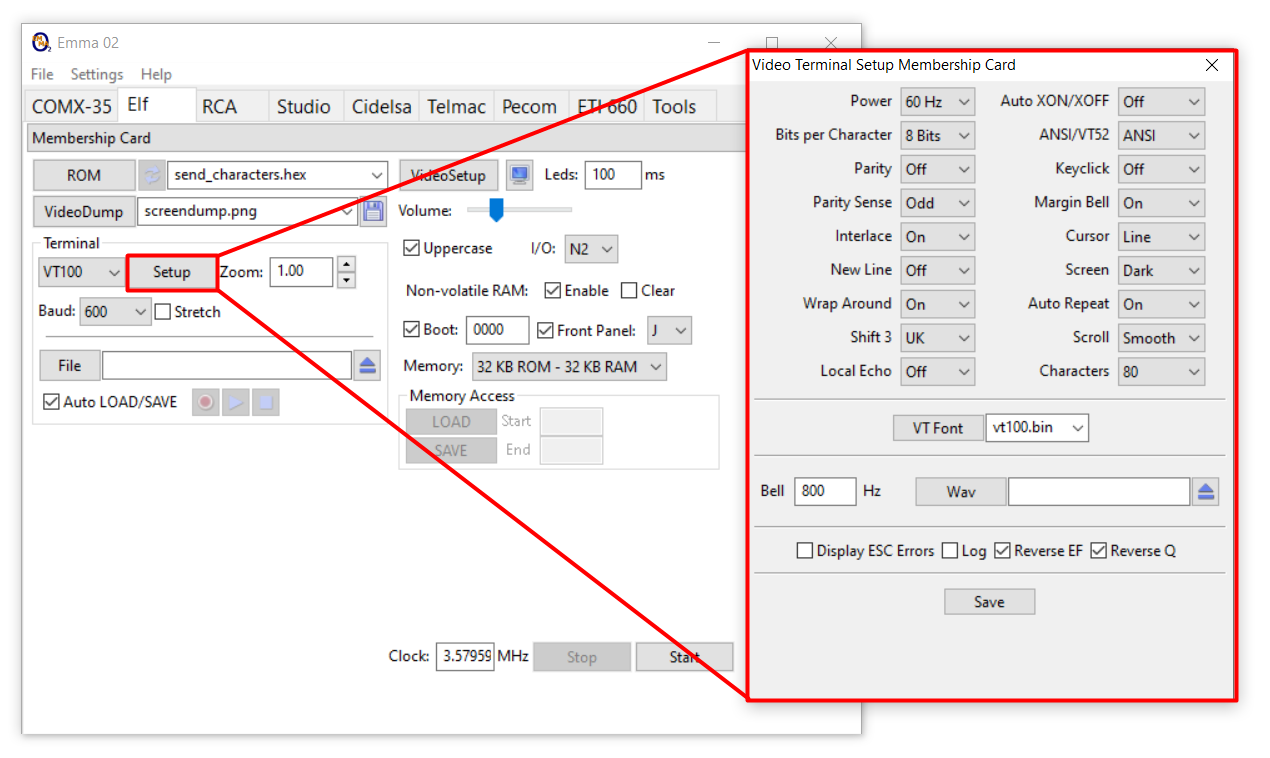
\includegraphics[width=1\textwidth]{./imagenes/config_emma02_sis_min.png}
  \caption{Configuración utilizada en el simulador Emma02}
  \label{F:config_emma02_sis_min}
\end{figure}

En la figura~\ref{F:prog_4_resultados} puede observarse el resultado obtenido tanto en simulación como en el sistema mínimo construido. Los resultados obtenidos en ambos casos fueron acordes a lo esperado. La configuración en Tera Term fue de 600~baudios, 8~bits para tamaño de datos, sin bit de paridad y con dos bits de parada.

\begin{figure}[H]
\centering
\subfloat[Resultado obtenido en Emma02]{
	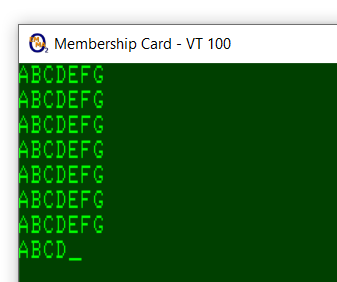
\includegraphics[width=0.45\textwidth]{./imagenes/programa_4_emma02.png}
	\label{F:programa_4_emma02}}
\quad
\subfloat[\centering Resultado experimental obtenido con el sistema mínimo]{
	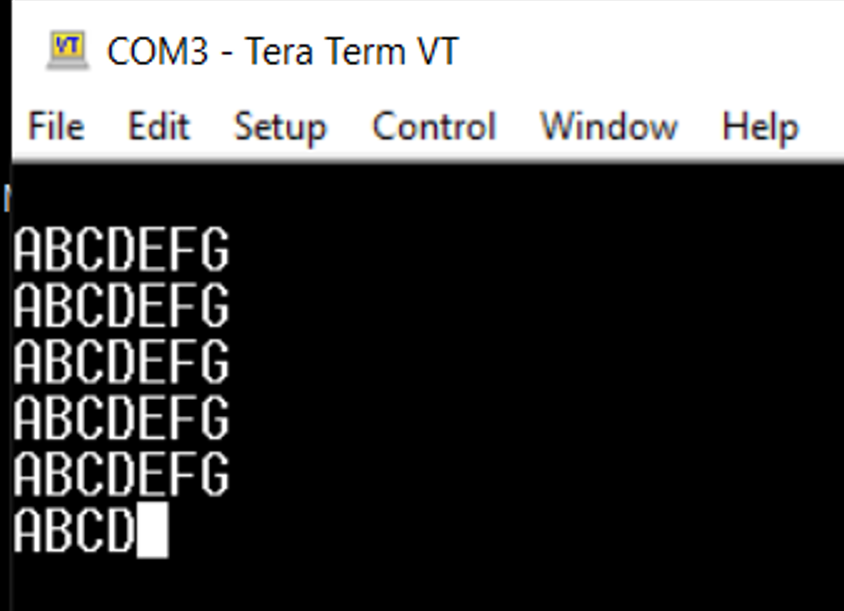
\includegraphics[width=0.45\textwidth]{./imagenes/programa_4_real.png}
	\label{F:programa_4_real}}
\caption{Resultados de la ejecución del programa 4}
\label{F:prog_4_resultados}
\end{figure}

%% agregar captura de los caracteres obtenidos en esta parte, simulación y real juntos
%% explicar que el terminal externo es una computadora aparte corriendo Tera Term

\section{Programador}
Para insertar los programas diseñados en la memoria EEPROM fue requerido el diseño de un circuito programador. El diseño adoptado se basa en un Arduino Nano. El software utilizado para el mismo no es de nuestra autoría, se encuentra disponible en la red \cite{pagina_programador}; aun así, se tuvieron que realizar modificaciones, con ayuda de programación en Python, para obtener un resultado satisfactorio, ya que luego de compilar un programa se disponía del mismo en formato Intel y este debía ser interpretado antes de pasarlo al Arduino que se encargaría de grabar la memoria.



Finalmente, el resultado obtenido con el programador sirvió para realizar unos ensayos y grabar memoria, sin embargo, debido a su dificultad de operación se terminó descartando y se reemplazó por el uso del programador presentado en la sección~\ref{C:Programador}. Aun así, por haberse construido, se presenta el esquemático del circuito en la figura~\ref{F:EsquemaProg} y una fotografía del resultado obtenido en la figura~\ref{F:PlacaProg}.

\begin{figure}[ht]
  \centering
  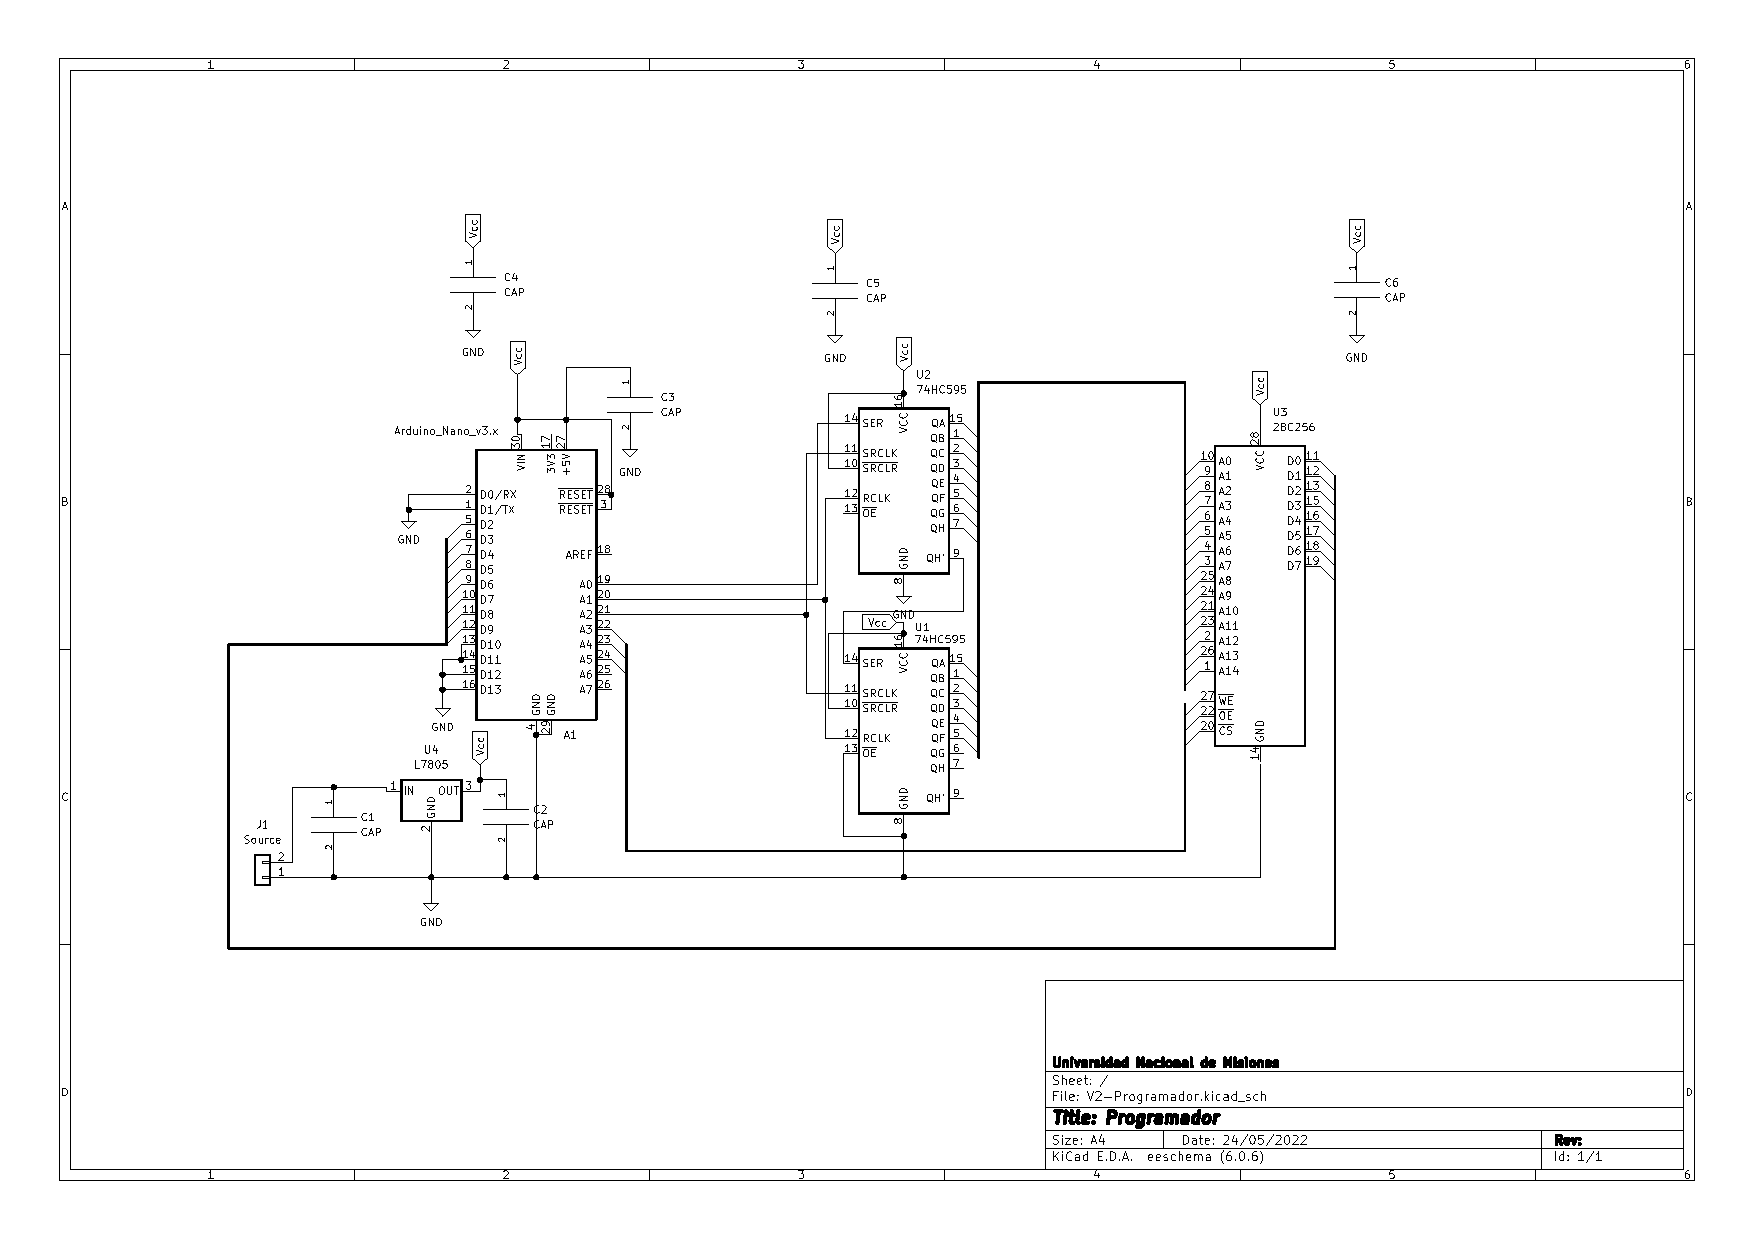
\includegraphics[width=1.2\textwidth, angle=90]{./imagenes/EsqProg.pdf}
  \caption{Esquema de programador}
  \label{F:EsquemaProg}
\end{figure}


\begin{figure}[ht]
\centering
\subfloat[Pista diseñada para Programador]{
	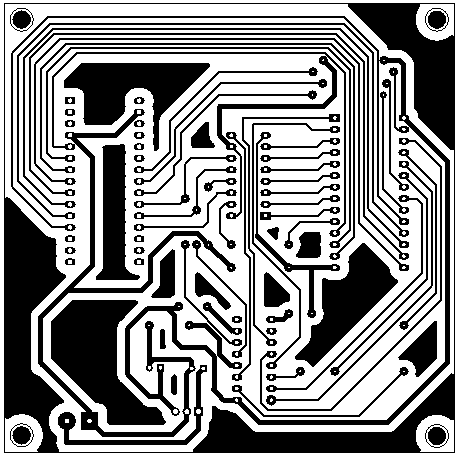
\includegraphics[width=0.52\textwidth]{./imagenes/PistaProg.png}
	\label{F:PistaProg}}

\subfloat[Máscara de componentes de Programador]{
	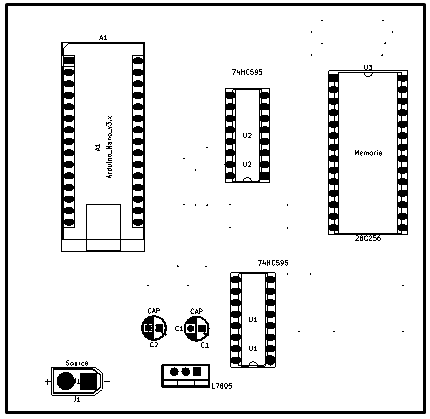
\includegraphics[width=0.51\textwidth]{./imagenes/MascProg.png}
	\label{F:MascaraProg}}
\caption{Placa PCB diseñada para el programador de memoria}
\label{F:PlacaProg}
\end{figure}

